% Fig 8: Adjacent-subcarrier correlation heatmap (schematic)
\begin{figure}[t]
\centering
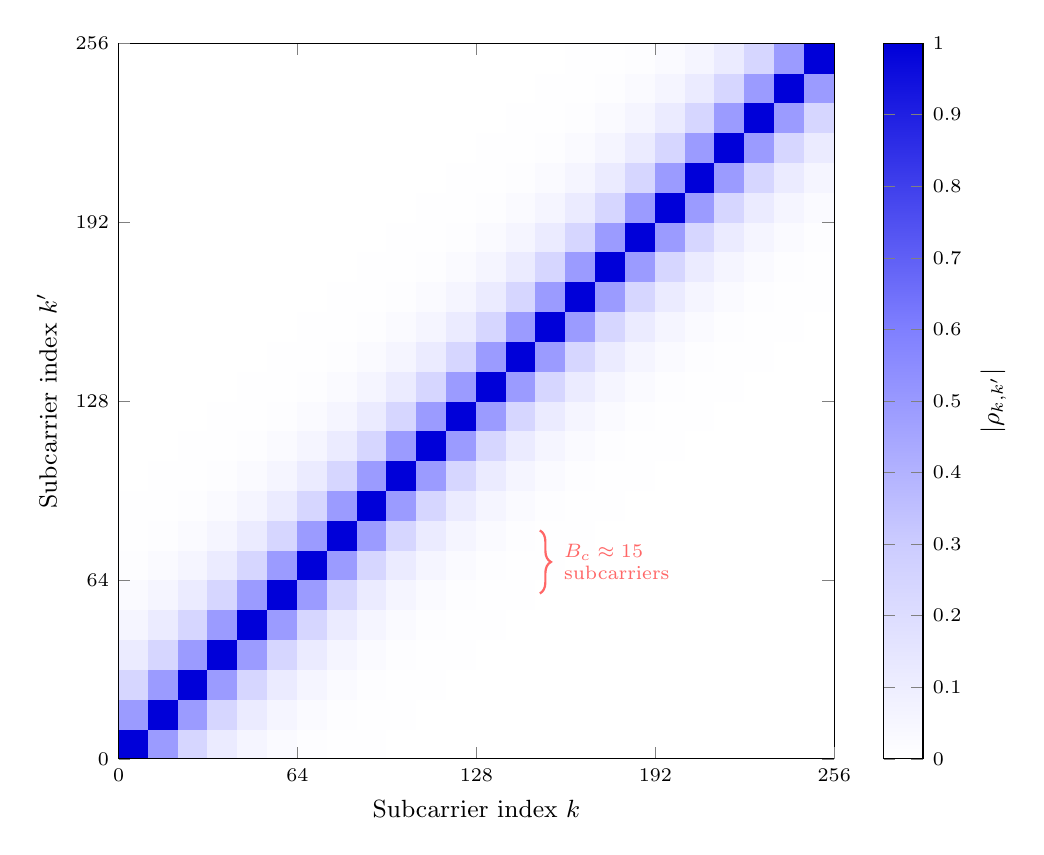
\begin{tikzpicture}
\begin{axis}[
  width=0.88\columnwidth,
  height=0.88\columnwidth,
  xlabel={Subcarrier index $k$},
  ylabel={Subcarrier index $k'$},
  xlabel style={font=\small},
  ylabel style={font=\small},
  xticklabel style={font=\scriptsize},
  yticklabel style={font=\scriptsize},
  xtick={0,64,128,192,256},
  ytick={0,64,128,192,256},
  xmin=0, xmax=256,
  ymin=0, ymax=256,
  colorbar,
  colorbar style={
    ylabel={$|\rho_{k,k'}|$},
    ylabel style={font=\small},
    yticklabel style={font=\scriptsize},
  },
  colormap={bluegrad}{
    color(0)=(white)
    color(0.3)=(blue!20)
    color(0.6)=(blue!50)
    color(1)=(blue!85!black)
  },
  view={0}{90},
  point meta min=0,
  point meta max=1,
]
% Correlation decays exponentially with subcarrier distance
% Coherence bandwidth ~ 15 subcarriers at 20 MHz indoor
\addplot3[surf, shader=flat corner, samples=25, domain=0:256, y domain=0:256]
  {exp(-abs(x-y)/15)};
\end{axis}

% Annotation: brace for coherence bandwidth
\draw[decorate, decoration={brace, amplitude=4pt, mirror}, thick, red!60]
  (5.35, 2.1) -- (5.35, 2.9)
  node[midway, right=5pt, font=\scriptsize, text=red!60, align=left] {$B_c \approx 15$\\subcarriers};
\end{tikzpicture}
\caption{Schematic subcarrier correlation structure. Phase LSB correlation $|\rho_{k,k'}| \approx e^{-|k-k'|/B_c}$ decays with subcarrier spacing, where $B_c \approx 15$ subcarriers is the coherence bandwidth at 20~MHz indoors. The near-diagonal banding drives the gap between per-byte (6.36) and final (5.50~bpb) min-entropy. Mitigations: extract every $n$-th subcarrier or apply whitening.}
\label{fig:correlation-heatmap}
\end{figure}
